\documentclass[
    xcolor={svgnames,dvipsnames},
    hyperref={colorlinks, citecolor=DeepPink4, linkcolor=DarkRed, urlcolor=DarkBlue}
    ]{beamer}  % for hardcopy add 'trans'


\mode<presentation>
{
  \usetheme{Singapore}
  % or ...
  \setbeamercovered{transparent}
  % or whatever (possibly just delete it)
}

%\usefonttheme{professionalfonts}
%\usepackage[english]{babel}
% or whatever
%\usepackage[latin1]{inputenc}
% or whatever
%\usepackage{times}
%\usepackage[T1]{fontenc}
% Or whatever. Note that the encoding and the font should match. If T1
% does not look nice, try deleting the line with the fontenc.

%\usepackage{fontspec}
%\setmonofont{CMU Typewriter Text}
%\setmonofont{Consolas}

\usepackage{fontspec} 
\usepackage[xcharter]{newtxmath}
\setmainfont{XCharter}
%\usepackage{unicode-math}
%\setmathfont{XCharter-Math.otf}
\setmonofont{DejaVu Sans Mono}[Scale=MatchLowercase] % provides unicode characters 



%%%%%%%%%%%%%%%%%%%%%% start my preamble %%%%%%%%%%%%%%%%%%%%%%

\addtobeamertemplate{navigation symbols}{}{%
    \usebeamerfont{footline}%
    \usebeamercolor[fg]{footline}%
    \hspace{1em}%
    \insertframenumber/\inserttotalframenumber
}


\usepackage{graphicx}
\usepackage{amsmath, amssymb, amsthm}
\usepackage{bbm}
\usepackage{mathrsfs}
\usepackage{xcolor}
\usepackage{fancyvrb}


% Quotes at start of chapters / sections
\usepackage{epigraph}  
%\renewcommand{\epigraphflush}{flushleft}
%\renewcommand{\sourceflush}{flushleft}
\renewcommand{\epigraphwidth}{6in}

%% Fonts

%\usepackage[T1]{fontenc}
\usepackage{mathpazo}
%\usepackage{fontspec}
%\defaultfontfeatures{Ligatures=TeX}
%\setsansfont[Scale=MatchLowercase]{DejaVu Sans}
%\setmonofont[Scale=MatchLowercase]{DejaVu Sans Mono}
%\setmathfont{Asana Math}
%\setmainfont{Optima}
%\setmathrm{Optima}
%\setboldmathrm[BoldFont={Optima ExtraBlack}]{Optima Bold}

% Some colors

\definecolor{aquamarine}{RGB}{69,139,116}
\definecolor{midnightblue}{RGB}{25,25,112}
\definecolor{darkslategrey}{RGB}{47,79,79}
\definecolor{darkorange4}{RGB}{139,90,0}
\definecolor{dogerblue}{RGB}{24,116,205}
\definecolor{blue2}{RGB}{0,0,238}
\definecolor{bg}{rgb}{0.95,0.95,0.95}
\definecolor{DarkOrange1}{RGB}{255,127,0}
\definecolor{ForestGreen}{RGB}{34,139,34}
\definecolor{DarkRed}{RGB}{139, 0, 0}
\definecolor{DarkBlue}{RGB}{0, 0, 139}
\definecolor{Blue}{RGB}{0, 0, 255}
\definecolor{Brown}{RGB}{165,42,42}


\setlength{\parskip}{1.5ex plus0.5ex minus0.5ex}

%\renewcommand{\baselinestretch}{1.05}
%\setlength{\parskip}{1.5ex plus0.5ex minus0.5ex}
%\setlength{\parindent}{0pt}

% Typesetting code
\definecolor{bg}{rgb}{0.95,0.95,0.95}
\usepackage{minted}
\setminted{mathescape, frame=lines, framesep=3mm}
\usemintedstyle{friendly}
%\newminted{python}{}
%\newminted{c}{mathescape,frame=lines,framesep=4mm,bgcolor=bg}
%\newminted{java}{mathescape,frame=lines,framesep=4mm,bgcolor=bg}
%\newminted{julia}{mathescape,frame=lines,framesep=4mm,bgcolor=bg}
%\newminted{ipython}{mathescape,frame=lines,framesep=4mm,bgcolor=bg}


\newcommand{\Fact}{\textcolor{Brown}{\bf Fact. }}
\newcommand{\Facts}{\textcolor{Brown}{\bf Facts }}
\newcommand{\keya}{\textcolor{turquois4}{\bf Key Idea. }}
\newcommand{\Factnodot}{\textcolor{Brown}{\bf Fact }}
\newcommand{\Eg}{\textcolor{ForestGreen}{Example. }}
\newcommand{\Egs}{\textcolor{ForestGreen}{Examples. }}
\newcommand{\Ex}{{\bf Ex. }}



\renewcommand{\theFancyVerbLine}{\sffamily
    \textcolor[rgb]{0.5,0.5,1.0}{\scriptsize {\arabic{FancyVerbLine}}}}

\newcommand{\navy}[1]{\textcolor{Blue}{\bf #1}}
\newcommand{\brown}[1]{\textcolor{Brown}{\sf #1}}
\newcommand{\green}[1]{\textcolor{ForestGreen}{\sf #1}}
\newcommand{\blue}[1]{\textcolor{Blue}{\sf #1}}
\newcommand{\navymth}[1]{\textcolor{Blue}{#1}}
\newcommand{\emp}[1]{\textcolor{DarkOrange1}{\bf #1}}
\newcommand{\red}[1]{\textcolor{Red}{\bf #1}}

% Symbols, redefines, etc.

\newcommand{\code}[1]{\texttt{#1}}

\newcommand{\argmax}{\operatornamewithlimits{argmax}}
\newcommand{\argmin}{\operatornamewithlimits{argmin}}

\DeclareMathOperator{\cl}{cl}
\DeclareMathOperator{\interior}{int}
\DeclareMathOperator{\Prob}{Prob}
\DeclareMathOperator{\determinant}{det}
\DeclareMathOperator{\trace}{trace}
\DeclareMathOperator{\Span}{span}
\DeclareMathOperator{\rank}{rank}
\DeclareMathOperator{\cov}{cov}
\DeclareMathOperator{\corr}{corr}
\DeclareMathOperator{\var}{var}
\DeclareMathOperator{\mse}{mse}
\DeclareMathOperator{\se}{se}
\DeclareMathOperator{\row}{row}
\DeclareMathOperator{\col}{col}
\DeclareMathOperator{\range}{rng}
\DeclareMathOperator{\dimension}{dim}
\DeclareMathOperator{\bias}{bias}


% mics short cuts and symbols
\newcommand{\st}{\ensuremath{\ \mathrm{s.t.}\ }}
\newcommand{\setntn}[2]{ \{ #1 : #2 \} }
\newcommand{\cf}[1]{ \lstinline|#1| }
\newcommand{\fore}{\therefore \quad}
\newcommand{\tod}{\stackrel { d } {\to} }
\newcommand{\toprob}{\stackrel { p } {\to} }
\newcommand{\toms}{\stackrel { ms } {\to} }
\newcommand{\eqdist}{\stackrel {\textrm{ \scriptsize{d} }} {=} }
\newcommand{\iidsim}{\stackrel {\textrm{ {\sc iid }}} {\sim} }
\newcommand{\1}{\mathbbm 1}
\newcommand{\dee}{\,{\rm d}}
\newcommand{\given}{\, | \,}
\newcommand{\la}{\langle}
\newcommand{\ra}{\rangle}

\newcommand{\boldA}{\mathbf A}
\newcommand{\boldB}{\mathbf B}
\newcommand{\boldC}{\mathbf C}
\newcommand{\boldD}{\mathbf D}
\newcommand{\boldM}{\mathbf M}
\newcommand{\boldP}{\mathbf P}
\newcommand{\boldQ}{\mathbf Q}
\newcommand{\boldI}{\mathbf I}
\newcommand{\boldX}{\mathbf X}
\newcommand{\boldY}{\mathbf Y}
\newcommand{\boldZ}{\mathbf Z}

\newcommand{\bSigmaX}{ {\boldsymbol \Sigma_{\hboldbeta}} }
\newcommand{\hbSigmaX}{ \mathbf{\hat \Sigma_{\hboldbeta}} }

\newcommand{\RR}{\mathbbm R}
\newcommand{\NN}{\mathbbm N}
\newcommand{\PP}{\mathbbm P}
\newcommand{\EE}{\mathbbm E \,}
\newcommand{\XX}{\mathbbm X}
\newcommand{\ZZ}{\mathbbm Z}
\newcommand{\QQ}{\mathbbm Q}

\newcommand{\fF}{\mathcal F}
\newcommand{\dD}{\mathcal D}
\newcommand{\lL}{\mathcal L}
\newcommand{\gG}{\mathcal G}
\newcommand{\hH}{\mathcal H}
\newcommand{\nN}{\mathcal N}
\newcommand{\pP}{\mathcal P}




\title{Introduction to HPC with Python: \\
    History, Trends and Future Directions} 

\author{John Stachurski}


\date{October 2023}


\begin{document}

\begin{frame}
  \titlepage
\end{frame}







\begin{frame}
    \frametitle{Outline}

    \begin{itemize}
        \item Trends in scientific computing
        \vspace{0.5em}
        \item Likely future directions
        \vspace{0.5em}
        \item Hands-on computing with Python + NumPy + Numba + JAX
    \end{itemize}

\end{frame}



\begin{frame}
    \frametitle{A (very) short history of scientific computing}


    General purpose scientific computing environments:

        \vspace{0.5em}
        \vspace{0.5em}
    \begin{enumerate}
        \item Fortran \& C / C++ 
        \vspace{0.5em}
        \vspace{0.5em}
        \item MATLAB \& (Python + NumPy)
        \vspace{0.5em}
        \vspace{0.5em}
        \item Julia \& (Python + Numba) 
        \vspace{0.5em}
        \vspace{0.5em}
        \item Python + Google JAX 
    \end{enumerate}

\end{frame}



\begin{frame}[fragile]
    \frametitle{Fortran \& C --- static types and AOT compilers}

    {\small
    \begin{minted}{c}
#include <stdio.h>
int main() {
    int x = 1 + 1;
    printf("1 + 1 = %d\n", x);
    return 0;
}   
    \end{minted}
    }


    {\small
    \begin{minted}{fortran}
PROGRAM ONE_PLUS_ONE  
INTEGER :: X = 1 + 1 
PRINT *, '1 + 1 = ', X
END PROGRAM ONE_PLUS_ONE 
    \end{minted}
    }

\end{frame}


\begin{frame}
    

    Pros

    \begin{itemize}
        \item fast  --- on a single thread
    \end{itemize}


    \vspace{0.5em}

    Cons

    \begin{itemize}
        \item tedious to write
        \item lack of portability
        \item hard to debug
        \item hard to parallelize
        \item low interactivity
    \end{itemize}

\end{frame}



\begin{frame}
    \frametitle{Phase 2: MATLAB}

    
    \begin{figure}
       \begin{center} % l b r t
        \scalebox{.6}{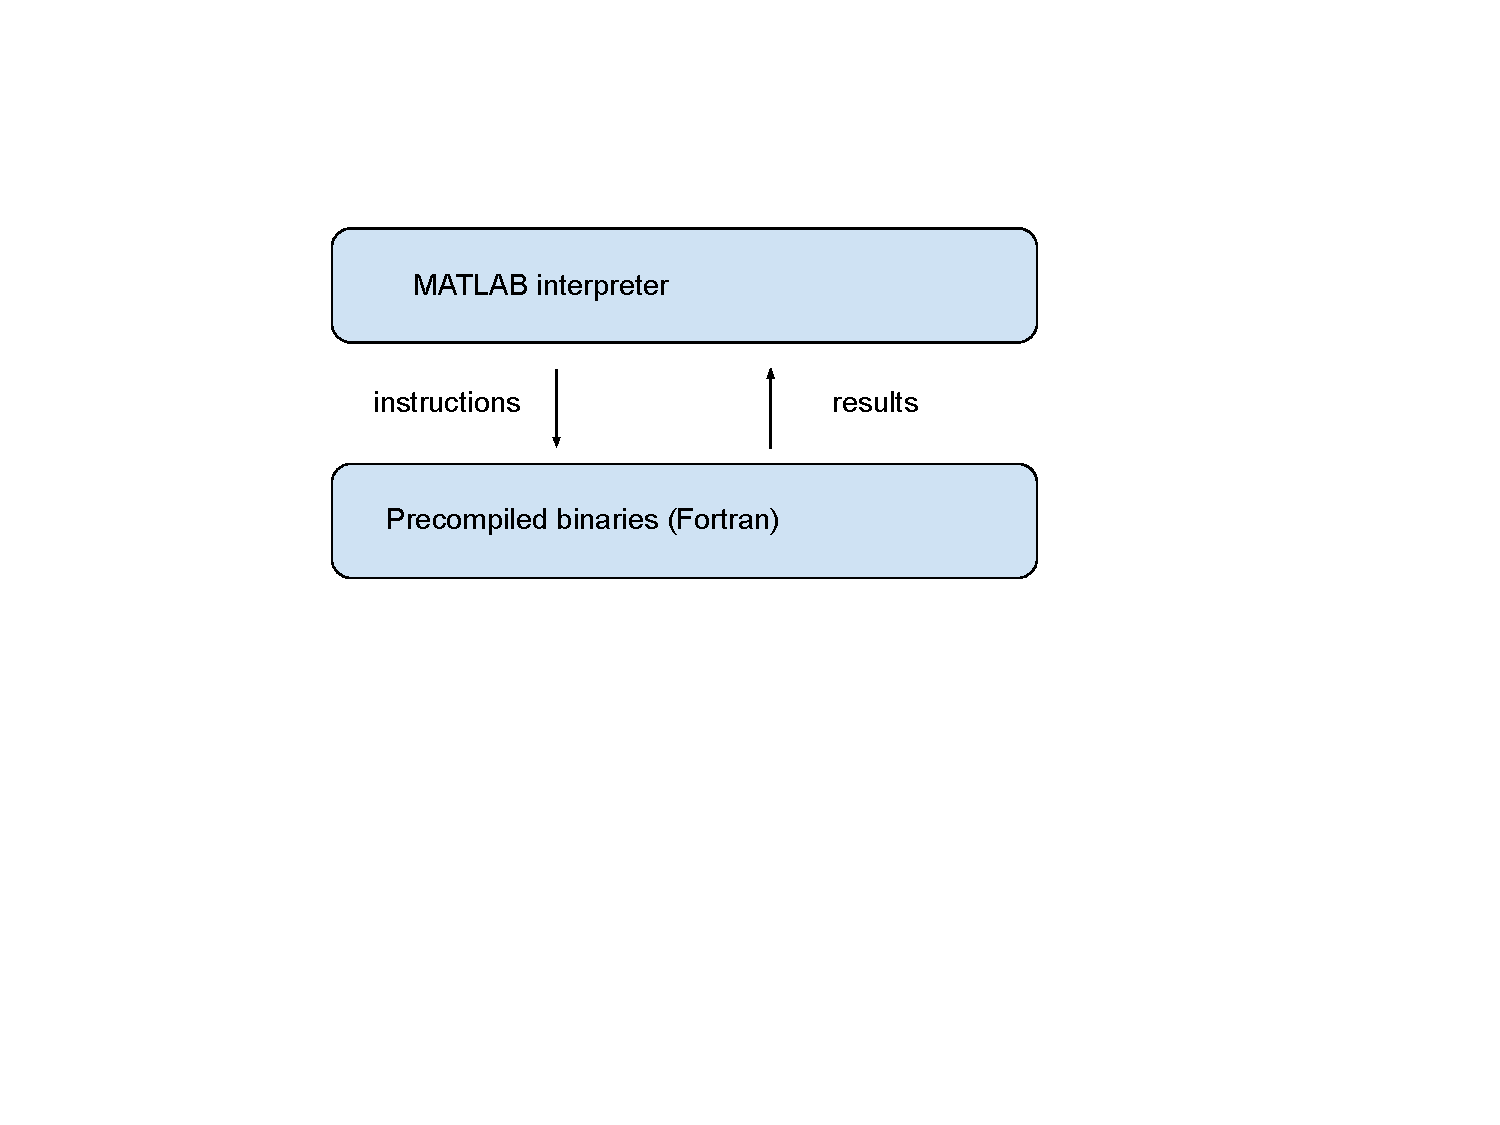
\includegraphics[trim={2cm 8cm 6cm 3cm},clip]{matlab.pdf}}
       \end{center}
    \end{figure}


\end{frame}




\begin{frame}
    \frametitle{Phase 2A: Python + NumPy}

    
    \begin{figure}
       \begin{center} % l b r t
        \scalebox{.6}{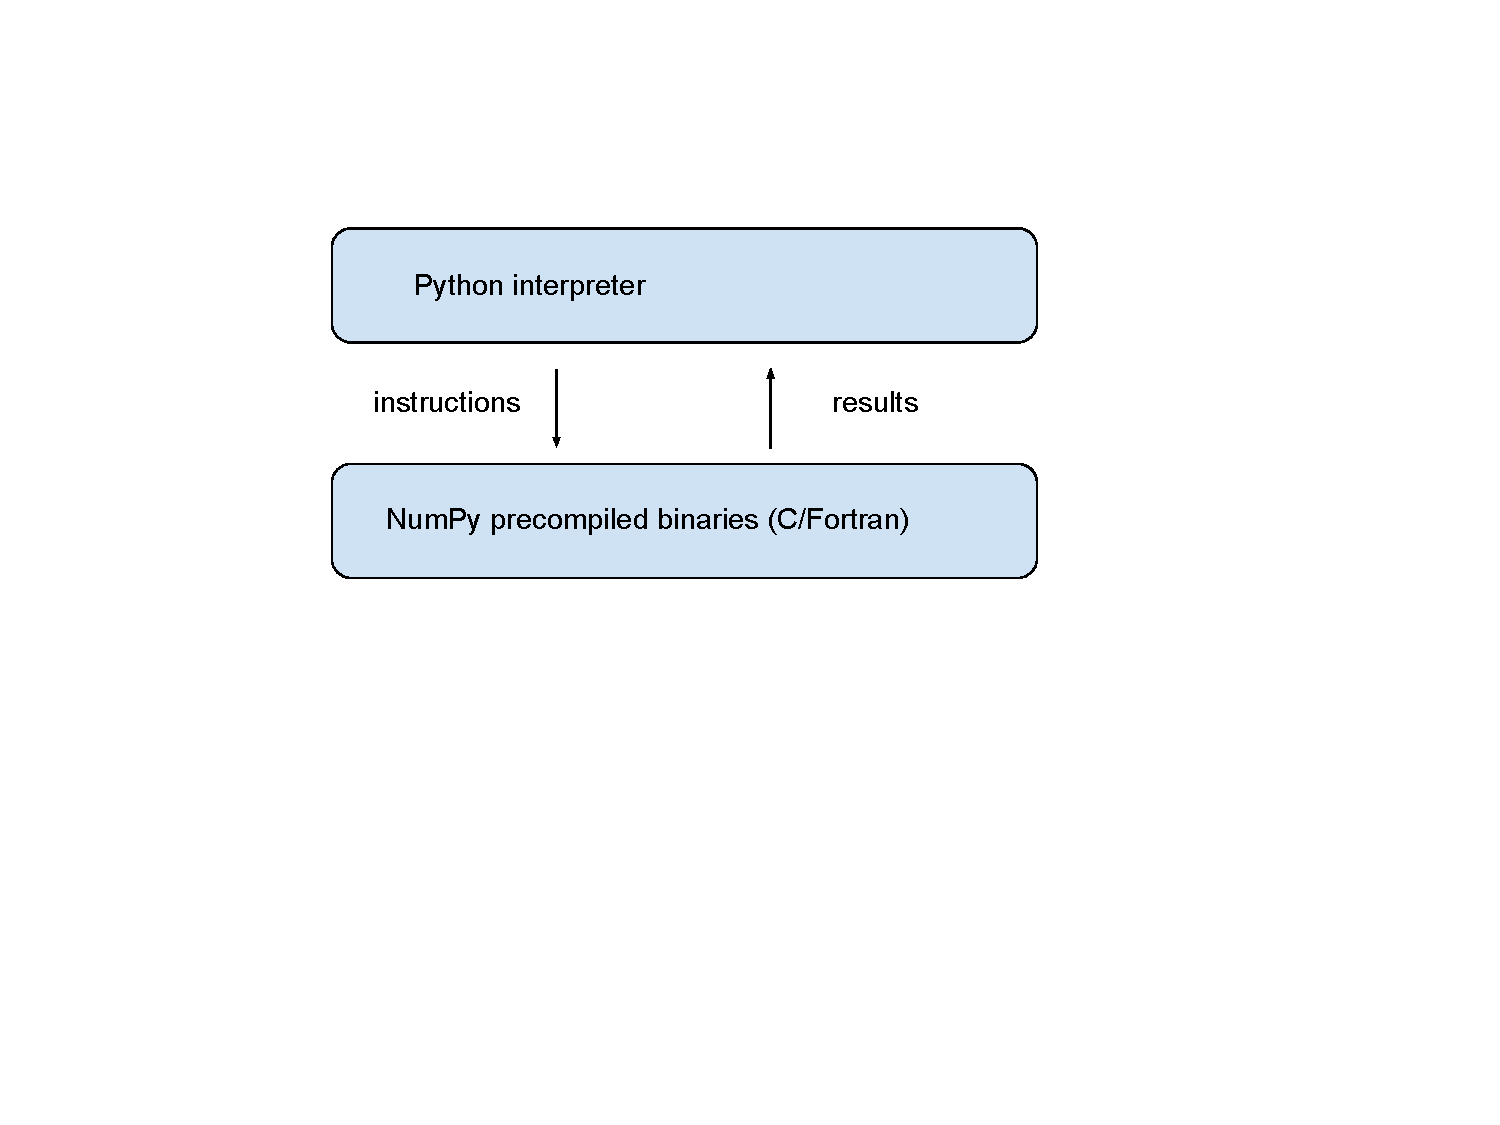
\includegraphics[trim={2cm 8cm 6cm 3cm},clip]{numpy.pdf}}
       \end{center}
    \end{figure}


\end{frame}



\begin{frame}[fragile]
    \frametitle{Phase 3: Julia --- rise of the JIT compilers}
    
    \begin{minted}{julia}

function quad(x0, α, n)
    x = x0
    for i in 1:(n-1)
        x = α * x * (1 - x)
    end
    return x
end

quad(0.2, 4.0, 10_000_000)
    \end{minted}

\end{frame}


\begin{frame}[fragile]
    \frametitle{Phase 3 continued: Python + Numba copy Julia}
    
    \begin{minted}{python}
from numba import jit

@jit
def quad(x0, α, n):
    x = x0
    for i in range(n-1):
        x = α * x * (1 - x)
    return x

quad(0.2, 4.0, 10_000_000)
    \end{minted}

\end{frame}

\begin{frame}
    \frametitle{Phase 4: AI-driven scientific computing}

    Core elements
    %
    \begin{itemize}
        \item JIT-compilers
        \vspace{0.5em}
        \item automatic differentiation
        \vspace{0.5em}
        \item parallelization (CPUs / GPUs / TPUs)
    \end{itemize}

    Key players
    %
    \begin{itemize}
        \item TensorFlow, PyTorch 
        \vspace{0.5em}
        \item Google JAX
        \vspace{0.5em}
        \item Mojo?
    \end{itemize}
    
\end{frame}

\begin{frame}
    

    AI / machine learning: minimizing differentiable loss functions
    
    \begin{figure}
       \begin{center}
        \scalebox{0.5}{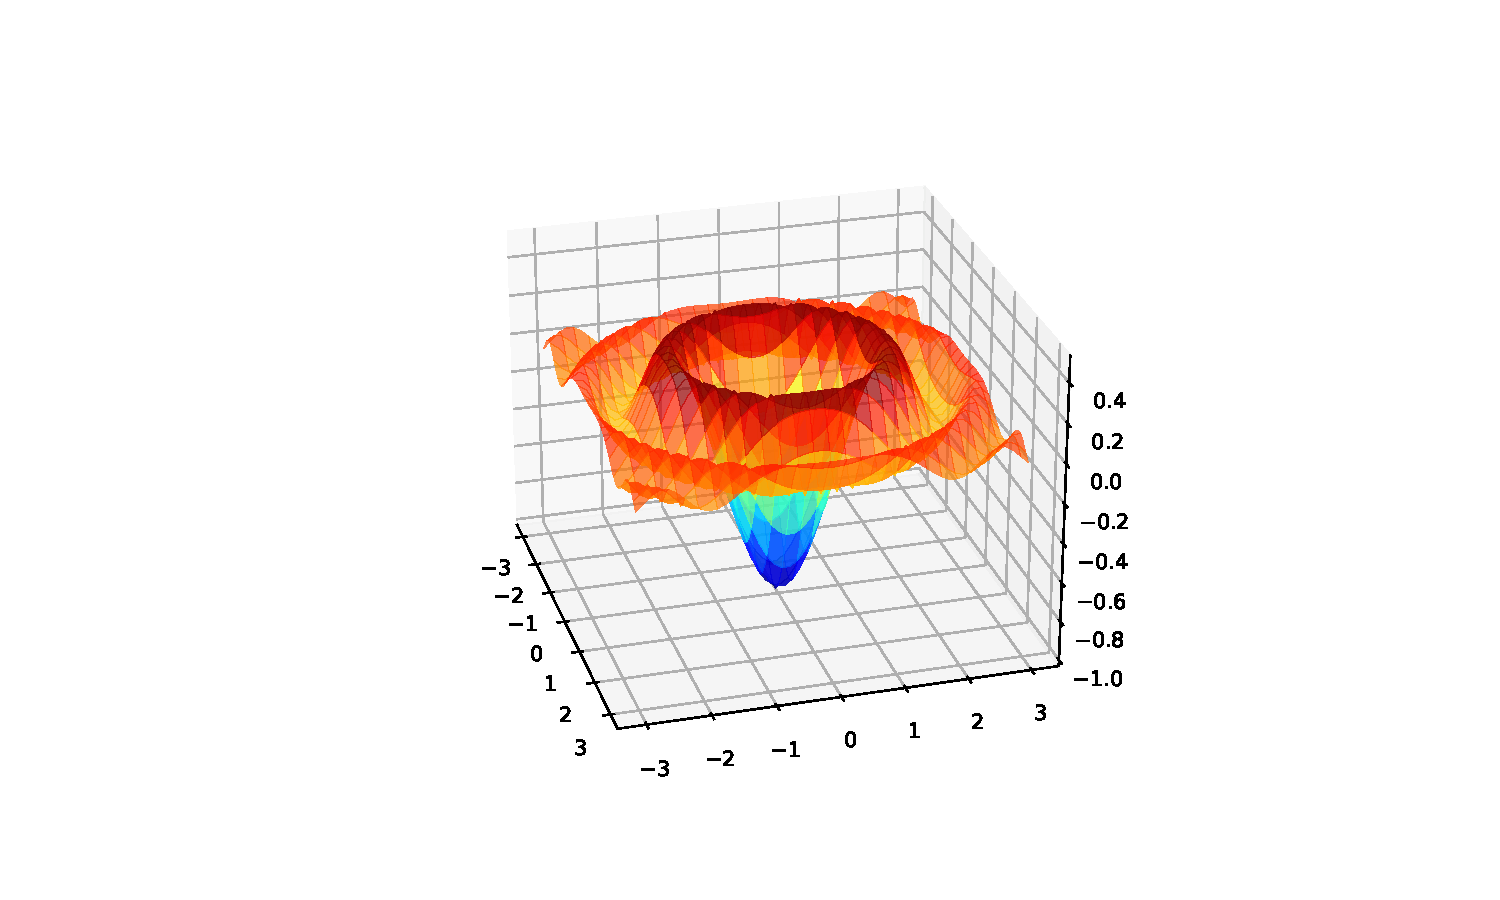
\includegraphics[trim={2cm 2cm 2cm 3cm},clip]{loss.pdf}}
       \end{center}
    \end{figure}


\end{frame}


\begin{frame}

    Stack Overflow Trends

    \begin{figure}
       \begin{center}
        \scalebox{0.25}{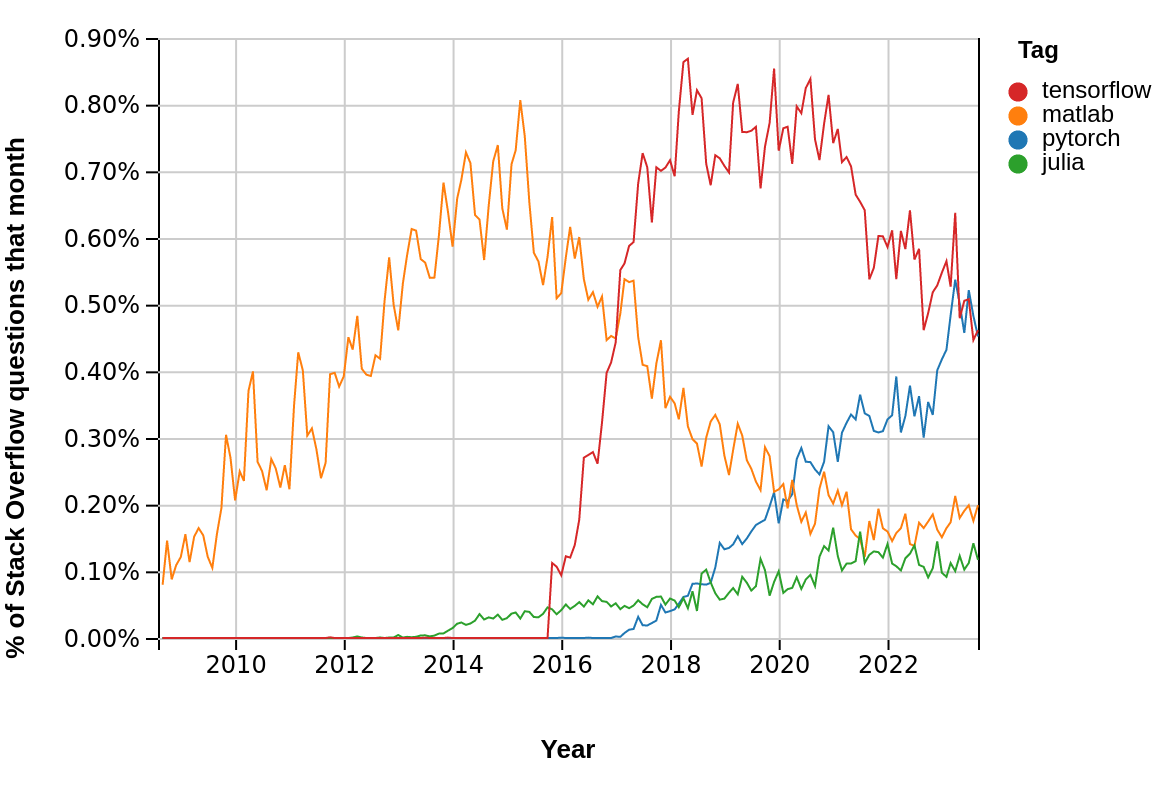
\includegraphics{pvr.png}}
       \end{center}
    \end{figure}

\end{frame}



\begin{frame}
    
    Sample code

    \url{https://github.com/QuantEcon/columbia_2023/notebooks}

\end{frame}


\end{document}


